\documentclass[]{spie}  %>>> use for US letter paper
%\documentclass[a4paper]{spie}  %>>> use this instead for A4 paper
%\documentclass[nocompress]{spie}  %>>> to avoid compression of citations

\renewcommand{\baselinestretch}{1.0} % Change to 1.65 for double spacing
 
\usepackage{amsmath,amsfonts,amssymb}
\usepackage{graphicx}
\usepackage[colorlinks=true, allcolors=blue]{hyperref}

\title{Simulating the LSST OCS for Conducting Survey Simulations Using the LSST Scheduler}

\author[a]{Michael A. Reuter*}
\author[b]{Kem H. Cook}
\author[a]{Francisco Delgado}
\author[a]{Catherine E. Petry}
\author[c]{Stephen T. Ridgway}
\affil[a]{LSST, 950 N Cherry Ave, Tucson, AZ USA}
\affil[b]{Cook Astronomical Consulting, San Ramon, CA USA}
\affil[c]{National Optical Astronomy Observatory, 950 N Cherry Ave, Tucson, AZ USA}

\authorinfo{Further author information: (Send correspondence to M.A.R.)\\M.A.R.: E-mail: mareuter@lsst.org}

% Option to view page numbers
\pagestyle{empty} % change to \pagestyle{plain} for page numbers   
\setcounter{page}{301} % Set start page numbering at e.g. 301
 
\begin{document} 
\maketitle

\begin{abstract}
The Operations Simulator was used to prototype the LSST Scheduler. Currently, the Scheduler is being developed separately to interface with the LSST Observatory Control System (OCS). A new Simulator is under concurrent development to adjust to this new architecture. This requires a package simulating enough of the OCS to allow execution of realistic schedules. This new package is called the Simulated OCS (SOCS). In this paper we will detail the SOCS construction plan, package structure, LSST communication middleware platform use, provide some interesting use cases that the separated architecture allows and the software engineering practices used in development.
\end{abstract}

% Include a list of keywords after the abstract 
\keywords{LSST, simulations, observing strategy}

\section{INTRODUCTION}
\label{sec:intro}  % \label{} allows reference to this section

In both research and development phase of the LSST project prior to the construction award in August 2014 and the subsequent years afterwards saw the successful development and testing of the Operations Simulator (OpSim) \cite{2014SPIE.9149E..0GD}\cite{2014SPIE.9150E..15D}\cite{2013AAS...22124703S}\cite{2010SPIE.7737E..0ZR}\cite{2010AAS...21540105K}\cite{2009AAS...21346004C}\cite{2007AAS...21113703P}\cite{2006SPIE.6270E..1DD}\cite{2006AAS...209.8604P}\cite{2005AAS...207.2626C}\cite{2004AAS...20510809C} . OpSim is a software application that contains an environment simulation using data from the actual LSST site, a fully detailed kinematic telescope and camera model, configuration parameters for controlling the science driven requirements, and the prototype version of the LSST Scheduler. OpSim has been tuned to produce the current LSST baseline survey and some alternate survey strategies\cite{Cook_SPIE2016}. 

While OpSim has been successful at producing survey strategy scenarios, the Scheduler is entwined within the code base. When LSST begins operations, it will require the Scheduler to perform the duties of determining the next targets to observe while interfacing with the LSST's Observatory Control System (OCS)\cite{Daly_SPIE2016}. The Scheduler will use the LSST communication middleware\cite{Mills_SPIE2016} project which is layer upon the Data Distribution Service (DDS) architecture. DDS is a publish/subscribe system in common use for communication between components of complex systems. 

With the requirements stated above, the project decided to separate the Scheduler\cite{Delgado_SPIE2016} into its own code base so that an effective deliverable can be provided.  In order to continue running simulations with the refactored Scheduler, a new harness is being created that utilizes the same DDS infrastructure to communicate with the Scheduler. This new project is called the Simulated Observatory Control System (SOCS). SOCS is not a high fidelity simulation of the entire OCS, but just enough of it to get the Scheduler to complete an entire survey. The combination of SOCS and the Scheduler is still collectively called the OpSim version 4 (OpSim4) whereas the older Operations Simulator is now referred to as OpSim version 3 (OpSim3). The schematic representations for both versions are shown in Figure~\ref{fig:opsim}.

\begin{figure} [ht]
  	\begin{center}
  		\begin{tabular}{c} 
  			\includegraphics[height=4cm]{Opsimv3.png}
  			\includegraphics[height=4cm]{Opsimv4.png}
  		\end{tabular}
  	\end{center}
  	\caption[What is this?] 
  	{ \label{fig:opsim} 
  		The left figure schematically shows the operational bounding box for OpSim version 3. This clearly indicates the buried nature of the Scheduler within the confines of OpSim. The right figure schematically shows the operational bounding box for OpSim version 4. This shows the newly separated nature of the two components which allow for development and usage flexibility.}
\end{figure} 

\section{CONSTRUCTION}
\label{sec:construction}

Since SOCS and the Scheduler have interdependent functionality, the developed construction plans are tightly coupled. 

\section{CONSTRUCTION AND DESIGN}

The design of SOCS inherits from lessons learned in building OpSim3. Among those is a desire for a more modular approach to the software with some parts of the Application Programming Interface (API) available for use outside the main steering program. Figure~\ref{fig:comparch} shows the top-level component diagram. It contains both module definitions as well as information flow between components and between SOCS and the Scheduler.

\begin{figure} [ht]
\begin{center}
\begin{tabular}{c}
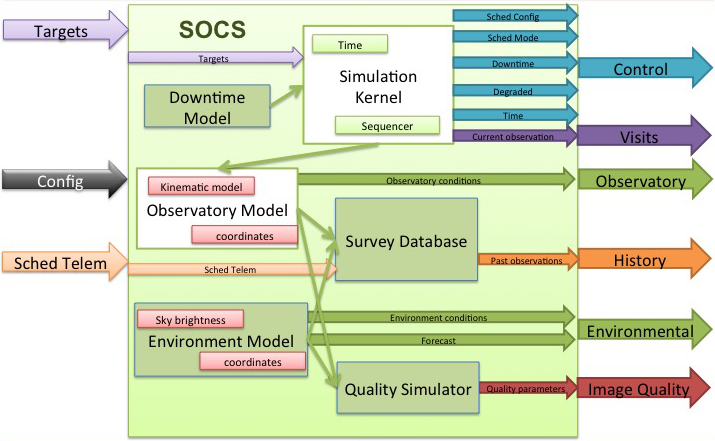
\includegraphics[height=5cm]{CompArch.png}
\end{tabular}
\end{center}
\caption[example]
{ \label{fig:comparch} 
This diagram shows the block level components for the SOCS design as well as the information flow both internal and external to SOCS.}
\end{figure}

\subsection{Modules}

The code will be divided into modules with each one characterized by a particular set of behaviors and responsibilities for the system. Descriptions of the modules are given in the following sections.

\subsubsection{Simulation Kernel}

The Simulation Kernel, designated hereafter as Kernel, is responsible for the main control flow of the simulator. There is a Simulator class which handles that orchestration of the different steps within the survey simulation. The TimeHandler class is clock for running the survey simulation. The timestamps provided by this class are updated faster than real time since it does not have to wait for any subsystem to return information. However, the timestamps run from the beginning of the survey until its finish. Finally, there is the Sequencer which mimics some of the behavior of its OCS counterpart. This class is responsible for performing the observation cycle on the requested target that was given by the Scheduler. 

\subsubsection{Observatory Model}

The Observatory Model contains the representation of the "real" LSST observatory. It uses as an aggregate the Observatory Model from the Scheduler. The Scheduler's model will always be an ideal version of the real observatory. However, the SOCS Observatory model is constructed for allowing perturbations of the various model parameters. This allows for testing of engineering scenarios of degraded observatory performance. This module also contains container classes used for gathering information about the Observatory for inclusion in the survey database. 

\subsubsection{Survey Database}

This module handles the creation and interactions for the generated survey database. It contains functions that specify the information content of the different tables and then construct the actual instances of those tables. There are functions that also aid in the ability to map data from DDS topics and other SOCS information structures onto the appropriate columns for a given table. The SocsDB class is the main orchestrator of survey database interactions. It is responsible for creating the database, gathering the data for output and actually performing the database writes. The system is designed to output either a MySQL or a SQLite database.

\subsubsection{Environmental Model}

The Environmental Model will contain classes that handle digesting and distributing environmental information, such as weather and astronomical sky conditions, to the Scheduler. This module is due to reach development status about the time this paper is presented at the conference, so specific details are not available. Much of the information that will be provided to the Scheduler will be available to SOCS in a digested format. Most of information will be provided to the Scheduler as a sky grid of some granularity rather than a single number for the entire sky.

\subsubsection{Quality Simulator}

While this module has not reached the development stage of the construction plan, it also has a known set of functionality. The module will contain classes that mimic some the behavior of the Data Management Level 1 products. The main focus is the image feedback on things like seeing, transparency and other quality metrics. This system will be engineered to provide some mechanism for occasionally making images that do not meet the constraints of a good visit. This information will be fed back to the Scheduler and the winning proposals for that visit will need to determine how the quality factors effect their completeness requirements.

\subsubsection{SAL}

While this module is not on the diagram, it is a useful nonetheless as it helps handle the interaction between other classes and the LSST middleware's Software Abstraction Layer (SAL). The class, called SalManager, allows for the ease creation and setting of publish and subscribe topics that are the backbone of the communication between SOCS and the Scheduler. The class also provides an easy mechanism for performing the actual publishing of topics and receiving the subscribed topics.

\subsubsection{Configuration}

This is another module not on the diagram, but one that keeps  the baseline LSST survey configuration. It uses a configuration system that is available from the LSST Data Management software stack\cite{2015arXiv151207914J}. The classes contain the appropriate configuration parameters for the baseline survey and the configuration system provides a mechanism to override those values without changing the code. There are also classes which interface the configuration parameters to the configuration DDS topics that need to be passed to the Scheduler.

\subsection{Information Flow}

We will now describe the content of the information flow for SOCS.

\subsubsection{Configuration}
\label{sec:code-config}


\begin{figure} [ht]
	\begin{center}
		\begin{tabular}{c}
			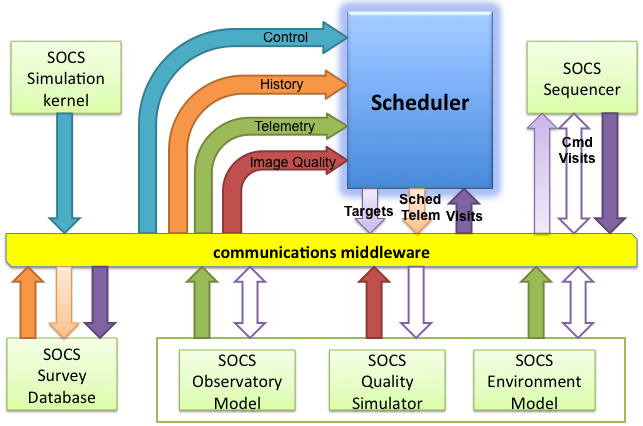
\includegraphics[height=5cm]{CommFlow.png}
		\end{tabular}
	\end{center}
	\caption[example]
	{ \label{fig:commflow} 
		This diagram shows the DDS communication pathways between the SOCS and Scheduler systems.}
\end{figure}

Figure~\ref*{fig:commflow} is an exact replica of a diagram showing the interaction of the Scheduler and the OCS with SOCS simulating OCS functions. The job of SOCS is to provide all of the needed inputs to the Scheduler shown in this diagram. Central to this diagram is the communications middleware, which currently is DDS. The details of this interface are described in the Scheduler interface document. Key to the design of SOCS is the ability to simulate a survey either deterministically or with stochastic variation in a variety of outputs. This is needed to understand the behavior of simulated surveys when the Scheduler is not provided completely accurate environmental data due to rapid variation in the environment, and also when the Scheduler’s telescope model is not a completely accurate model of the real telescope.

\section{SOFTWARE ENGINEERING}

OpSim3 had a document detailing all of the functional and performance requirements for the developed system which included those for the Scheduler. The factorization of OpSim3 into the SOCS and Scheduler components necessitated a factorization of the requirements document into one for each resulting system. The SOCS requirements document was adjusted to account for the new role as the harness for driving the Scheduler and placed under LSST project level change control.

A development plan for SOCS was created containing incremental releases, with a specific set of capabilities and validation activities for each one. This plan is captured in JIRA\cite{JIRA} release epics and described at a high level in Primavera PMCS. The plan is coordinated with the release timeline of the Scheduler due to their heavy interdependence.

The detailed construction plan is also described in JIRA epics relating to each release epic, keeping track of individual tasks that mark the way to each release. Tracking the development process uses the LSST variant of Agile software development\cite{Kantor_SPIE2016}. The JIRA plan, releases, milestones and tasks are used periodically to report back to PMCS and to compute EVM, and organize the work of the development team.

The SOCS code is kept in a Github\cite{GitHub} git repository, following coding standards from Data Management and Systems Engineering Simulations about templates, interfaces, coding and unit tests. The SOCS code follows the basic tenants of the Test Driven Design philosophy of software development. TDD requires unit tests to be run during the implementation process at a fairly high frequency to uncover issues quickly. The baseline science survey configuration is also kept with the SOCS GitHub repository. 

More importantly, each SOCS release is integrated and tested with the LSST Scheduler and the combined efforts from both the Telescope and Site and Systems Engineering Simulations teams. The capabilities of SOCS to drive the Scheduler for implementing the LSST survey are validated with specialized tools (MAF) and the participation of the science collaborations.

\section{USE CASES}

The separation of the Scheduler from the simulation harness allows for efficient development. This means only one code base has to be maintained to serve the separate systems (OCS and SOCS). This separated approach and the use of a standard communication framework allow for some interesting use cases with respect to the SOCS/Scheduler combination. The main use case, the ability to run a full LSST survey, is oth cases are predicated off the fact the configuration of the Scheduler that is running the LSST during operations can be injected into a new instance of the Scheduler. The new instance can be driven by SOCS to perform different scenarios while leaving the operating Scheduler unaffected. One scenario is advancing the Scheduler through a given time window in order to publish a list of targets that the LSST will visit within the caveats of environmental and instrumental conditions. Another scenario is to take the current Scheduler state and fast forward through the remaining survey to evaluate the efficiency based off the current progress. This mechanism can also be used to evaluate alternate scenarios for the survey, such as new proposals, proposals being finished or alternate configuration parameters.

\section{SUMMARY}

In this paper, we have shown the necessity for refactoring OpSim3 into the LSST Scheduler and SOCS which is known collectively as OpSim4. We presented the construction plan and architecture design for SOCS including information flow. We provided evidence of the software engineering practices applied during the code development of SOCS. Lastly, we presented some use cases that demonstrated the unique capabilities of this separated system. 

\acknowledgments % equivalent to \section*{ACKNOWLEDGMENTS}       

Financial support for LSST comes from the National Science Foundation (NSF) through Cooperative Agreement No. 1258333, the Department of Energy (DOE) Office of Science under Contract No. DE-AC02-76SF00515, and private funding raised by the LSST Corporation. The NSF-funded LSST Project Office for construction was established as an operating center under management of the Association of Universities for Research in Astronomy (AURA).  The DOE-funded effort to build the LSST camera is managed by the SLAC National Accelerator Laboratory (SLAC).    

% References
\bibliography{SimObsConSysSPIE991183} % bibliography data in report.bib
\bibliographystyle{spiebib} % makes bibtex use spiebib.bst

\end{document} 
